\renewcommand{\sectionTitle}{Arquitectura de Hardware}
\titlespacing*{\section}{0pt}{1.5\baselineskip}{2\baselineskip}
\titlespacing*{\subsection}{0pt}{1.5\baselineskip}{1\baselineskip}


\section{\sectionTitle}
\label{sec:section4}

\begin{figure}[H]
    \centering
    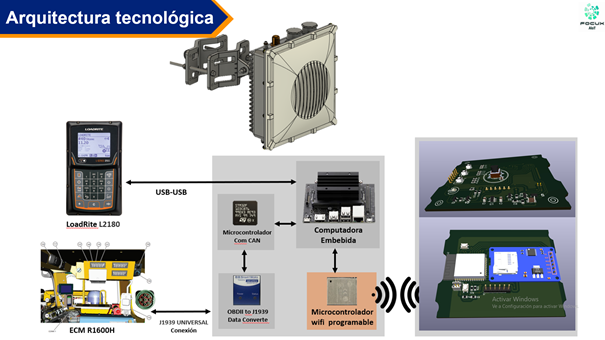
\includegraphics[height=2in]{images/general_arquitectura.png}
    \captionsetup{font=footnotesize}
    \caption{Arquitectura Tecnologica}
    \label{fig:img5_1}
\end{figure}


% 5.1
\subsection{Edge AIoT Box}
\label{subsection:subsec5_1}

\begin{figure}[H]
    \centering
    \includegraphics[height=2in]{images/edge_isometrico.png}
    \captionsetup{font=footnotesize}
    \caption{Vista externa Edge AIoT Box}
    \label{fig:img5_2}
\end{figure}

\begin{figure}[H]
    \centering
    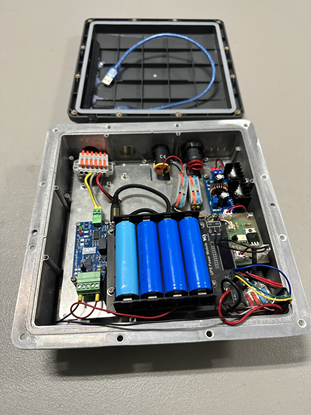
\includegraphics[height=2in]{images/edge_inside.png}
    \captionsetup{font=footnotesize}
    \caption{Vista interna Edge AIoT Box}
    \label{fig:img5_3}
\end{figure}

%5.1.1
\subsubsection{UPS Power Module}
\label{subsection:subsubsec5_1_1}
\paragraph{Descripcion General}
El Módulo de alimentación UPS para Jetson Nano, fuente de alimentación ininterrumpida de 5 V, circuitos de protección de batería múltiple es capaz de cargar las baterías y proporcionar salida de energía al mismo tiempo desde una fuente de alimentación externa.
Cambia automáticamente la salida de las baterías si la fuente de alimentación externa no está disponible, mantiene el sistema funcionando sin problemas.

\paragraph{Caracteristicas principales}
\begin{itemize}
    \item Comunicación de bus I2C, monitoreando el voltaje, la corriente, la potencia y la capacidad restante de la batería en tiempo real.
    \item OLED de 0,91" para mostrar información como el voltaje de la batería, la dirección IP, el uso de RAM, etc.
    \item Circuitos de protección de batería múltiple:
    \begin{itemize}
        \item Proteccion contra sobrecarga/descarga
        \item Proteccion contra sobrecorriente
        \item Proteccion contra cortocircuito
        \item Proteccion contra voltaje inverso
        \item Carga balanceada
    \end{itemize} 
    \item Regulador integrado de 5 V, hasta 2,5 A de corriente de salida continua.
    \item Indicadores de advertencia de baterías, fácil de comprobar si la batería está conectada correctamente.
\end{itemize}

\paragraph{Especificaciones}
\begin{itemize}
    \item Voltaje de salida: 5V
    \item Cargador: 8,4 V 2A
    \item Bus de control: I2C
    \item Batería compatible: batería 18650 Li
    \item Dimensión: 113 mm x 79 mm
    \item Orificio de montaje: 2,5 mm
\end{itemize}

\begin{figure}[H]
    \centering
    \includegraphics[height=2in]{images/ups_diagram_top.png}
    \captionsetup{font=footnotesize}
    \caption{Vista superior del modulo UPS}
    \label{fig:img5_4}
\end{figure}

\begin{figure}[H]
    \centering
    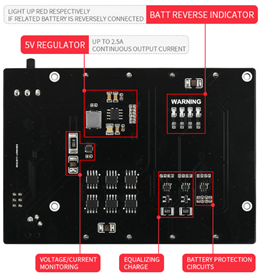
\includegraphics[height=2in]{images/ups_diagram_bottom.png}
    \captionsetup{font=footnotesize}
    \caption{Vista inferior del modulo UPS}
    \label{fig:img5_5}
\end{figure}


%5.1.2
\subsection{LED's}
\label{subsection:subsubsec5_1_2}

\paragraph{Descripcion}
Para indicar el funcionamiento del equipo Edge AIoT Box, se disponen de luces piloto de color rojo y verde. 
Dichas luces son compatibles con 24V o 12V, permitiendo ser energizadas por la maquinaria al que el equipo Edge AIoT Box estará conectado.
\begin{itemize}
    \item LED Rojo: Indica si el equipo está siendo energizado por la maquinaria. En caso no esté encendido 
    mientras la maquinaria está funcionando, indicaría una falla interna entre los cables de energía
    \item LED Verde: Indica si el equipo está almacenando datos de la maquinaria mediante parpadeo; esta luz queda encendida 
    sin parpadear mientras el equipo esté esperando datos provenientes de la maquinaria
\end{itemize}


%5.1.3
\subsection{Cable ODB2/J1939}
\label{subsection:subsubsec5_1_3}

\paragraph{Descripcion General}
Cable adaptador OBD2 de 9 pines a 16 pines: este cable adaptador J1939 a OBD2 puede evitar la línea de derivación original del vehículo original. 

\paragraph{Especificaciones}
\begin{table}[htb]
    \centering
    \begin{tabular}{|g|c|c|}
      \hline
      \textbf{Header 1} & \textbf{Header 2} & \textbf{Header 3} \\
      \hline
      Row 1, Column 1 & Row 1, Column 2 & Row 1, Column 3 \\
      \hline
      Row 2, Column 1 & Row 2, Column 2 & Row 2, Column 3 \\
      \hline
    \end{tabular}
    \captionsetup{font=footnotesize}
    \caption{Especificacion Cable ODB2/J1939}
    \label{tab:table_5_1_3}
  \end{table}
  
